\subsection{Adding Functional Reactive Programming}
\label{sec:step2_frp}
As shown in the first step, the need to handle $\Delta t$ explicitly can be quite messy, is inelegant and a potential source of errors, also the explicit handling of the state of an agent and its behavioural function is not very modular. We can solve both these weaknesses by switching to the functional reactive programming paradigm (FRP), because it allows to express systems with discrete and continuous time-semantics. In this step we are focusing on arrowized \cite{hughes_generalising_2000} FRP using the library Yampa \cite{hudak_arrows_2003}. In it, time is handled implicit, meaning it cannot be messed with, which is achieved by building the  whole system on the concept of signal functions (SF). A SF can be understood as a process over time and is technically a continuation which allows to capture state using closures. Both these fundamental features allow us to tackle the weaknesses of our first step and push our approach further towards a truly functional approach.

\subsubsection{Implementation}
We start by defining our agents now as a SF which receives the states of all agents as input and outputs the state of the agent:

\begin{HaskellCode}
type SIRAgent = SF [SIRState] SIRState 
\end{HaskellCode}

Now we can define the behaviour of an agent to be the following:

\begin{HaskellCode}
sirAgent :: RandomGen g => g -> SIRState -> SIRAgent
sirAgent g Susceptible = susceptibleAgent g
sirAgent g Infected    = infectedAgent g
sirAgent _ Recovered   = recoveredAgent
\end{HaskellCode}

Depending on the initial state we return one of three functions. Most notably is the difference that we are now passing a random-number generator instead of running in the Random Monad because signal functions as implemented in Yampa are not capable of being monadic. We see that the recovered agent ignores the random-number generator which is in accordance with the implementation in the previous step where it acts as a sink which returns constantly the same state:

\begin{HaskellCode}
recoveredAgent :: SIRAgent
recoveredAgent = arr (const Recovered)
\end{HaskellCode}

By using the Yampa combinator \textit{switch} we can change the behaviour of an agent when an event occurs which is much more elegant then the initial approach and much more expressive as it makes the change of behaviour at the occurrence of an event explicit. Thus a susceptible agent behaves as susceptible until it becomes infected. Upon infection an \textit{Event} is returned which results in switching into the \textit{infectedAgent} SF, which causes the agent to behave as an infected agent from that moment on. Instead of randomly drawing the number of contacts to make, we now follow a fundamentally different approach by using Yampas \textit{occasionally} function. It generates on average an event after the given time, so in each time-step we generate either a single event or no event. This requires a fundamental different approach in selecting the right $\Delta t$ and sampling the system as will be shown in results. 

\begin{HaskellCode}
susceptibleAgent :: RandomGen g => g -> SIRAgent
susceptibleAgent g = switch (susceptible g) (const (infectedAgent g))
  where
    susceptible :: RandomGen g => g -> SF [SIRState] (SIRState, Event ())
    susceptible g = proc as -> do
      makeContact <- occasionally g (1 / contactRate) () -< ()
      if isEvent makeContact
        then (do
          a <- drawRandomElemSF g -< as
          case a of
            Infected -> do
              i <- randomBoolSF g infectivity -< ()
              if i
                then returnA -< (Infected, Event ())
                else returnA -< (Susceptible, NoEvent)
             _       -> returnA -< (Susceptible, NoEvent))
        else returnA -< (Susceptible, NoEvent)
\end{HaskellCode}

We deal with randomness differently now and implement signal functions built on the \textit{noiseR} function provided by Yampa. This is another example of the stream character and statefulness of a signal function as it needs to keep track of the changed random-number generator internally through the use of continuations and closures. Here we provide the implementation of \textit{randomBoolSF}, drawRandomElemSF works similar but takes a list as input:

\begin{HaskellCode}
randomBoolSF :: RandomGen g => g -> Double -> SF () Bool
randomBoolSF g p = proc _ -> do
  r <- noiseR ((0, 1) :: (Double, Double)) g -< ()
  returnA -< (r <= p)
\end{HaskellCode}

The infected agent behaves as infected until it recovers on average after the illness duration after which it behaves as a recovered agent by switching into \textit{recoveredAgent}. As in the case of the susceptible agent, we use the \textit{occasionally} function to generate the event when the agent recovers. Note that the infected agent ignores the states of the other agents as its behaviour is completely independent of them.

\begin{HaskellCode}
infectedAgent :: RandomGen g => g -> SIRAgent
infectedAgent g = switch infected (const recoveredAgent)
  where
    infected :: SF [SIRState] (SIRState, Event ())
    infected = proc _ -> do
      recEvt <- occasionally g illnessDuration () -< ()
      let a = event Infected (const Recovered) recEvt
      returnA -< (a, recEvt)
\end{HaskellCode}

Running and stepping the simulation works now a bit differently. Yampa provides the function \textit{embed} which allows us to run a SF for a given number of steps where in each step one provides the $\Delta t$ and an optional input.

\begin{HaskellCode}
runSimulation :: RandomGen g => g -> Time -> DTime -> [SIRState] -> [[SIRState]]
runSimulation g t dt as = embed (stepSimulation sfs as) ((), dts)
  where
    steps     = floor (t / dt)
    dts       = replicate steps (dt, Nothing)
    n         = length as
    (rngs, _) = rngSplits g n [] -- creates unique RandomGens for each agent
    sfs       = map (\ (g', a) -> sirAgent g' a) (zip rngs as)
\end{HaskellCode}

What we now need to implement is a closed feedback-loop. Fortunately, \cite{nilsson_functional_2002}, \cite{courtney_yampa_2003} discusses implementing this in Yampa. The function \textit{stepSimulation} is an implementation of such a closed feedback-loop. It takes the current signal functions and states of all agents, runs them all in parallel and returns the new agent states of this step. Yampa provides the \textit{dpSwitch} combinator for running signal functions in parallel, which is quite involved and discussed more in-depth in section \ref{sec:background}. It allows us to recursively switch back into the \textit{stepSimulation} with the continuations and new states of all the agents after they were run in parallel.
In every step we generate a switching event using \textit{switchingEvt} which receives the outputs of all the run signal functions. It always returns an \textit{Event} with all the outputs which causes to switch into the continuation which is \textit{stepSimulation} itself . Note the use of \textit{notYet} which is required because in Yampa switching occurs immediately at $t = 0$.

\begin{HaskellCode}
stepSimulation :: [SIRAgent] -> [SIRState] -> SF () [SIRState]
stepSimulation sfs as =
    dpSwitch
      (\_ sfs' -> (map (\sf -> (as, sf)) sfs'))
      sfs
      (switchingEvt >>> notYet) 
      stepSimulation
  where
    switchingEvt :: SF ((), [SIRState]) (Event [SIRState])
    switchingEvt = arr (\ (_, newAs) -> Event newAs)
\end{HaskellCode}

\subsubsection{Results}
The function which drives the dynamics of our simulation is \textit{occasionally}, which randomly generates an event on average with a given rate following the exponential distribution. To arrive at the correct dynamics, this requires us to sample \textit{occasionally}, and thus the whole system, with small enough $\Delta t$ which matches the rate. If we choose a too large $\Delta t$, we loose events which will result in dynamics which do not approach the SD dynamics sufficiently enough, see Figure \ref{fig:sir_abs_dynamics_frp}.

\begin{figure}
\begin{center}
	\begin{tabular}{c c}
		\begin{subfigure}[b]{0.3\textwidth}
			\centering
			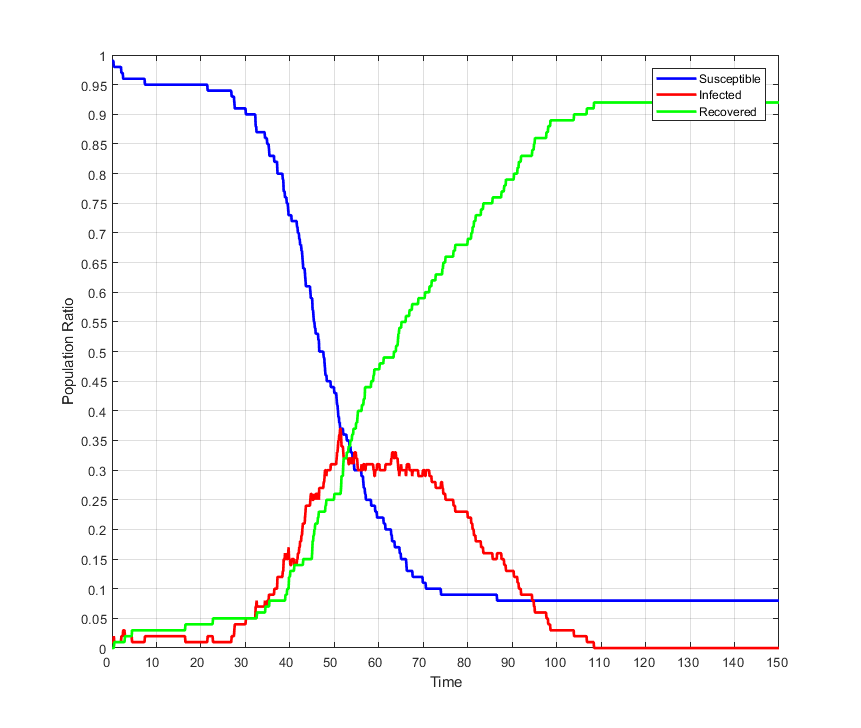
\includegraphics[width=1\textwidth, angle=0]{./fig/step2_yampa/SIR_100agents_150t_01dt.png}
			\caption{100 Agents, $\Delta t = 0.1$}
			\label{fig:sir_abs_approximating_01dt_100agents}
		\end{subfigure}
    	&
		\begin{subfigure}[b]{0.3\textwidth}
			\centering
			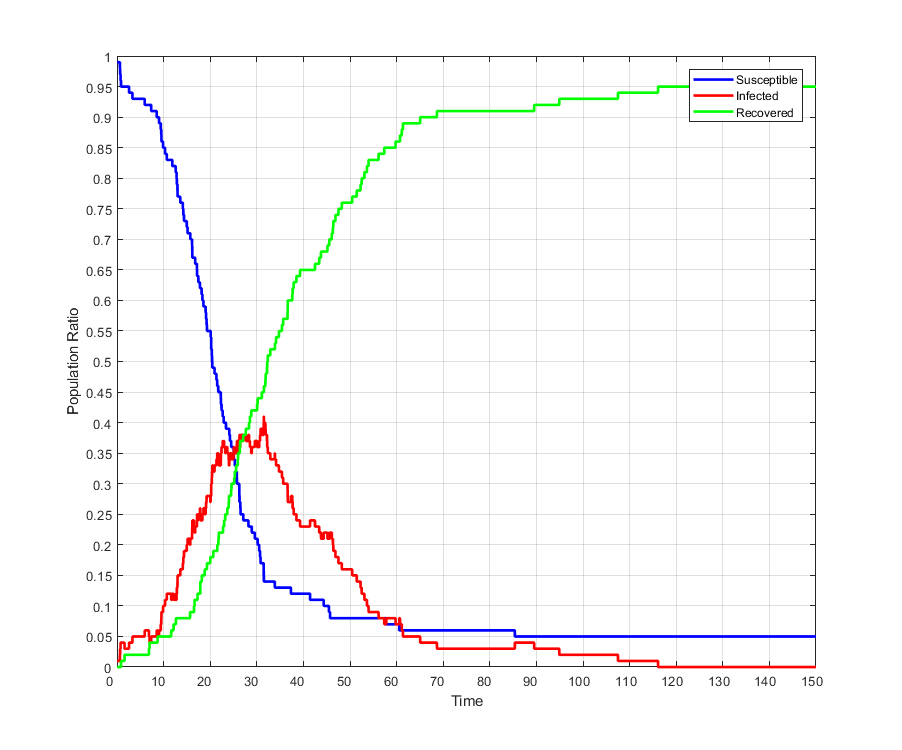
\includegraphics[width=1\textwidth, angle=0]{./fig/step2_yampa/SIR_100agents_150t_001dt.png}
			\caption{100 Agents, $\Delta t = 0.01$}
			\label{fig:sir_abs_approximating_001dt_500agents}
		\end{subfigure}
    	
    	\\
    	
		\begin{subfigure}[b]{0.3\textwidth}
			\centering
			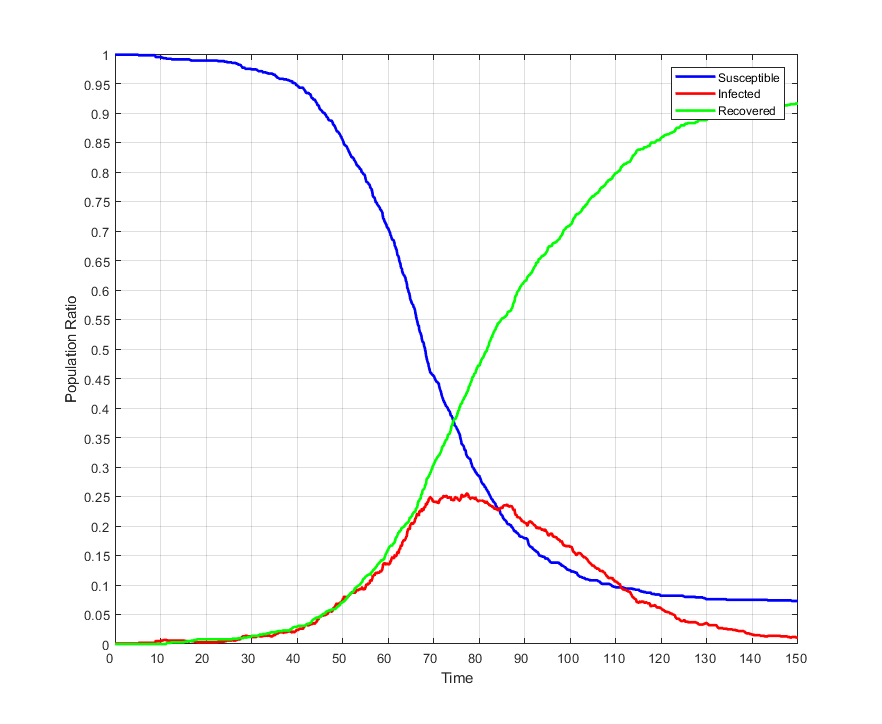
\includegraphics[width=1\textwidth, angle=0]{./fig/step2_yampa/SIR_1000agents_150t_01dt.png}
			\caption{1,000 Agents, $\Delta t = 0.1$}
			\label{fig:sir_abs_approximating_01dt_1000agents}
		\end{subfigure}
		& 
		\begin{subfigure}[b]{0.3\textwidth}
			\centering
			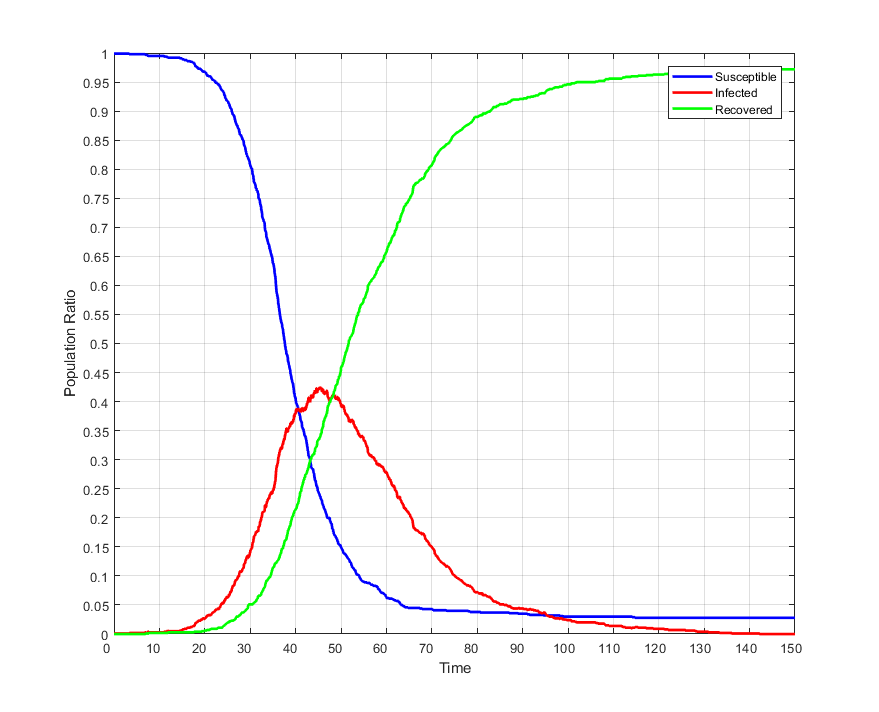
\includegraphics[width=1\textwidth, angle=0]{./fig/step2_yampa/SIR_1000agents_150t_001dt.png}
			\caption{1,000 Agents, $\Delta t = 0.01$}
			\label{fig:sir_abs_approximating_001dt_1000agents}
		\end{subfigure}
	\end{tabular}
	
	\caption{FRP simulation of SIR using agent-based approach. Population size of 100 and 1,000 with contact rate $\beta = \frac{1}{5}$, infection probability $\gamma = 0.05$, illness duration $\delta = 15$ with initially 1 infected agent. Simulation run for 150 time-steps with various $\Delta t$.} 
	\label{fig:sir_abs_dynamics_frp}
\end{center}
\end{figure}

Clearly by keeping the population size constant and just increasing the $\Delta t$ results in a closer approximation to the SD dynamics. Although the dynamics of Figure \ref{fig:sir_abs_approximating_001dt_1000agents} with 1000 agents and $\Delta t = 0.01$ look pretty close to SD, we are still not yet there. We would need to both decrease the sampling rate and increase the number of agents. Unfortunately at this point we are running into severe performance and memory problems because the whole system has to be sampled at an even finer $\Delta t$ whereas we only need to sample \textit{occasionally} with higher frequency. A possible solution would be to implement super-sampling which would allow us to run the whole simulation with $\Delta t = 1.0$ and only sample the \textit{occasionally} function with a much higher frequency. An approach would be to introduce a new function to Yampa which allows to super-sample other signal functions. 

\begin{HaskellCode}
superSampling :: Int -> SF a b -> SF a [b]
\end{HaskellCode}

It evaluates \textit{sf} for \textit{n} times, each with $\Delta t = \frac{\Delta t}{n}$ and the same input argument \textit{a} for all \textit{n} evaluations. At time 0 no super-sampling is performed and just a single output of \textit{sf} is calculated. A list of \textit{b} is returned with length of \textit{n} containing the result of the \textit{n} evaluations of \textit{sf}. If 0 or less super samples are requested exactly one is calculated. We could then just wrap the occasionally function which would then generate a list of events. We have investigated super-sampling more in-depth but have to leave this due to lack of space.

\subsubsection{Discussion}
By moving on to FRP using Yampa we made a huge improvement in clarity, expressivity and robustness of our implementation. State is now implicitly encoded, depending on which signal function is active. Also by using explicit time-semantics with \textit{occasionally} we can achieve extremely fine grained stochastics. Compared to drawing a random number of events we create only a single event or none at all. This requires to sample the system with a much smaller $\Delta t$: we are treating it as a truly continuous system, resulting in a hybrid SD/ABS approach.
Still we are not too happy about our approach as we feed back all agents states into every agent, something we want to omit in an agent-based simulation. We now move on to the next section in which we introduce a more general and much more controlled mechanism for feeding back agent-states. 